The first question we want to tackle is: how worse is the sparsity in an EPHS compared to a LSHS?
We show that, in general, the sparsity of an EPHS is arbitrarily worse.
Intuitively, this occurs when shortest and efficient paths are unrelated. 

\begin{proposition}
There is a family of networks with HD $1$ where the CHD can be arbitrarily large.
Additionally, the sparsity of the EPHS is also arbitrarily large.
\end{proposition}
\begin{proof}
Consider a directed graph $G$ defined as in Figure~\ref{fig:big_chd}.
There are $2n$ nodes $u_i,v_i$ and a special node $s$.
Every $u_i$ has two outgoing edges, one to $v_i$ with length $3$ and one to $s$ with length $1$.
Finally, $s$ has $n$ outgoing edges, one to every $v_i$ with length $1$.

\begin{figure}\caption{Graph with small HD and bi CHD}\label{fig:big_chd}
\begin{center}
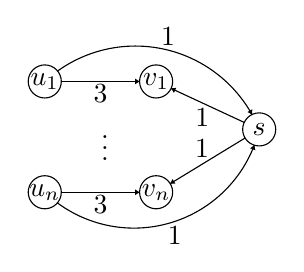
\begin{tikzpicture}[scale=0.07]
\tikzstyle{every node}+=[inner sep=0pt]
\draw [black] (18.5,-12.8) circle (3);
\draw (18.5,-12.8) node {$u_1$};
\draw [black] (38.7,-12.8) circle (3);
\draw (38.7,-12.8) node {$v_1$};
\draw [black] (18.5,-32.9) circle (3);
\draw (18.5,-32.9) node {$u_n$};
\draw [black] (38.7,-32.9) circle (3);
\draw (38.7,-32.9) node {$v_n$};
\draw (29.4,-23.4) node {$\vdots$} ;
\draw [black] (57.4,-21.5) circle (3);
\draw (57.4,-21.5) node {$s$};
\draw [black] (21.5,-12.8) -- (35.7,-12.8);
\fill [black] (35.7,-12.8) -- (34.9,-12.3) -- (34.9,-13.3);
\draw (28.6,-13.3) node [below] {$3$};
\draw [black] (21.5,-32.9) -- (35.7,-32.9);
\fill [black] (35.7,-32.9) -- (34.9,-32.4) -- (34.9,-33.4);
\draw (28.6,-33.4) node [below] {$3$};
\draw [black] (20.825,-10.907) arc (125.59934:29.18714:24.243);
\fill [black] (56.1,-18.8) -- (56.15,-17.85) -- (55.28,-18.34);
\draw (40.87,-6.38) node [above] {$1$};
\draw [black] (56.513,-24.364) arc (-20.88164:-126.45095:23.371);
\fill [black] (56.51,-24.36) -- (55.76,-24.93) -- (56.7,-25.29);
\draw (42.07,-39.01) node [below] {$1$};
\draw [black] (54.84,-23.06) -- (41.26,-31.34);
\fill [black] (41.26,-31.34) -- (42.2,-31.35) -- (41.68,-30.5);
\draw (47.05,-26.7) node [above] {$1$};
\draw [black] (54.68,-20.23) -- (41.42,-14.07);
\fill [black] (41.42,-14.07) -- (41.93,-14.86) -- (42.36,-13.95);
\draw (47.07,-17.66) node [below] {$1$};
\end{tikzpicture}
\end{center}
\end{figure}

Let us first determine the HD of $G$.
There are $2n$ shortest paths, namely $sv_i$ and $u_isv_i$ for different $i$.
We conclude that the HD is $1$, because it suffices to set $H_{v,r}=\crl{s}$ as the hitting set for every $r>0$ and $v\in V(G)$.

Now we add some costs and show that the CHD is at least $n$.
Let $c(u_iv_i)=0$ for every $i$ and set all other costs to $1$.
Note that the $1$-significant efficent paths intersecting the ball $B_s(2)$ are $u_iv_i$, which are all disjoint.
Therefore, the hitting set $H_{s,1}$ must contain at least $n$ elements.

We showed that the difference between HD and CHD is at least $n$.
We finish by noting that a similar argument shows that the sparsity of LSHS for $\calP$ is $1$, whereas the sparsity of EPHS is also lower bounded by $n$.
\end{proof}

\begin{remark}
Although this example shows the difference between HD and CHD, the reader may think that we are exploiting the maximum degree to our advantage.
This is not necessarily the case. 
In Section~\ref{app:generalhd}, where we discuss other notions of HD, we give a different, more involved, example that exhibits the same behaviour for even stronger versions of HD.
\end{remark}

It is conjectured that road networks have small HD.
Is there evidence to conjecture small CHD in these networks?
We show how doubling dimension plus an additional property, defined bellow, do imply a positive answer.
A path $P'$ \emph{partially witnesses} $P$ if $P'\subseteq P$ and $P'$ is ``long enough''.
Formally, we define the following relation for path systems.

\begin{definition}
Let $\beta\geq 0$.
We say that a path system $\calQ'$ is a $\beta$-witness of the path system $\calQ$ if, for every $Q\in\calQ$, exists $Q'\in\calQ'$ such that $Q'\subseteq Q$ and $\ell(Q')\geq 2^{-\beta}\ell(Q)$.
\end{definition}

We explore first when the system of shortest paths $\calP$ is a partial witness for the system of efficient paths $\PE$.
At an intuitive level, the partial witness property says that efficient and shortest paths are not completely different, i.e., if $Q$ is efficient, some fraction of $Q$ is shortest.
As a consequence, an important node hitting numerous paths in $\calP$, should also hit many paths in $\PE$.
The bad examples in Proposition~\ref{prop:treelike} exploit networks that do not have partial witnesses.
We stress that doubling dimension depends only on $G$ and $\ell$; the partial witness property depends on the interplay between $G$, $c$ and $\ell$.
For our result, we actually relax the partial witness property.
Notice that, in the statement of Theorem~\ref{theo:witness_doubling}, we ask only for long paths to be witnessed.

\begin{theorem}\label{theo:witness_doubling}
Assume that $G$ is $\alpha$-doubling and $\calP$ is a $\beta$-witness for $\PE_r$ for every $r\geq \frac{\log(\alpha^\beta h)}{2\log\Delta}$. \anote{There is no relation between the quantities $\alpha$ and $\Delta$ in the sense that neither bounds the other.}
If $(G,\ell)$ admits an $(h,r)$-LSHS for any $r$, then $(G,\ell,c)$ admits an $(\alpha^{\beta} h,r)$-EPHS for any $r$.
\end{theorem}
\begin{proof}
For any $r$, we need to construct a hitting set $C^E$ for $\calP_r^E$.
Assume first $r\geq \frac{\log(\alpha^\beta h)}{2\log\Delta}$.
Take $C$ as the hitting set for $\calP_{2^{-\beta}r}$, which is guaranteed to be sparse with respect to balls of radius $2^{-\beta+1}r$.
Define the desired set by
\[
C^E\defeq\{v\in C: v \text{ is in some $r$-efficient path} \}.
\]

Since $\calP$ is a $2^{-\beta}$-witness for $\PE_r$, $C^E$ is indeed a hitting set for $\PE_r$.
We are only left to prove the sparsity.
Take some $u\in V$, by doubling dimension we can cover $\Bf_{2r}(u)$ by at most $\alpha^\beta$ balls of radius $2^{-\beta+1}r$.
Each of these balls contains at most $h$ elements of $C$, therefore the sparsity is as claimed.
The argument for backward balls is identical.

Now we analyse the case $r< \frac{\log(\alpha^\beta h)}{2\log\Delta}$.
It is no longer true that the efficient paths are witnessed, but now the neigborhoods are small.
Take $C=V$ as the EPHS.
Clearly $C$ hits all the paths and the local sparsity is at most the size of the ball.
Using our assumption on $r$ and the fact that the lengths are integers, it follows that $\card{B_{2r}(v)}\leq\Delta^{2r}\leq\alpha^\beta h$. 
\end{proof}

\begin{remark}
The existence of a $\beta$-witness is not enough to bound the CHD.
Nevertheless, as discussed in Section~\ref{ssec:hldef}, the existence of $(h,r)$-LSHS already allows the construction of HL.
\end{remark}
